\section{Desarrollo/Análisis}
Inicialmente se hicieron todas las configuraciones necesarios con las referencias\cite{web5} dadas en clase. Hecho esto se logró sincronizar el microcontrolador con la página Edge Impulse. Esto permitió hacer uso del micrófono del Arduino Nano Ble 33 Sense y así comenzar con las grabaciones.

\begin{figure}[H]
\centering
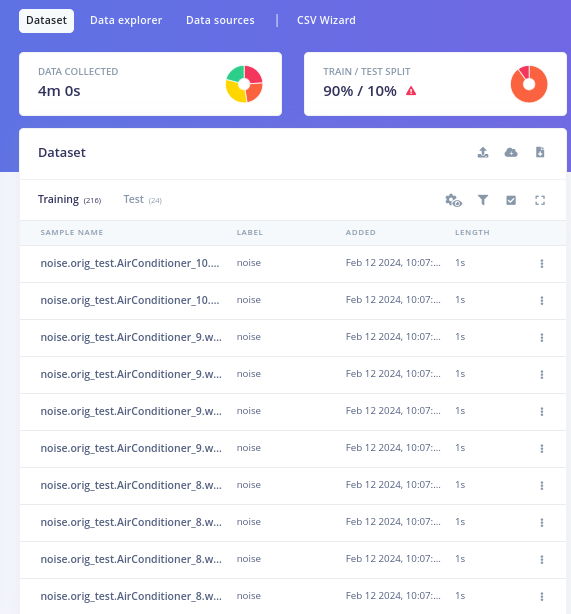
\includegraphics[width=.55\linewidth]{Img/data_set.png}
 \caption{Conjunto de datos.}
 \label{fig_dataset}
\end{figure}
En total de 240 muestras clasificadas por etiquetas.
\begin{itemize}
\item \texttt{OPEN\_TAG}.
    \begin{figure}[H]
    \centering
    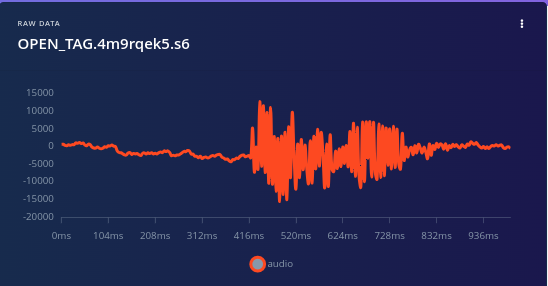
\includegraphics[width=.4\linewidth]{Img/open_tag.png}
    \caption{Espectro señal abrir.}
    \label{open_tag}
    \end{figure}
\item \texttt{CLOSE\_TAG}.
     \begin{figure}[H]
    \centering
    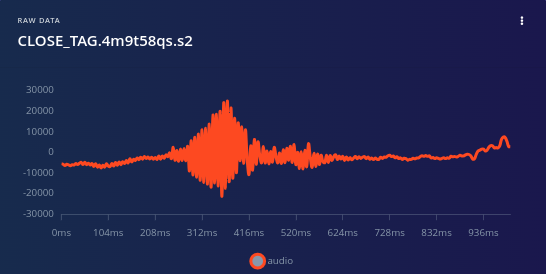
\includegraphics[width=.4\linewidth]{Img/close_tag.png}
    \caption{Espectro señal cierra.}
    \label{close_tag}
    \end{figure}
\item \texttt{NOISE}.
    \begin{figure}[H]
    \centering
    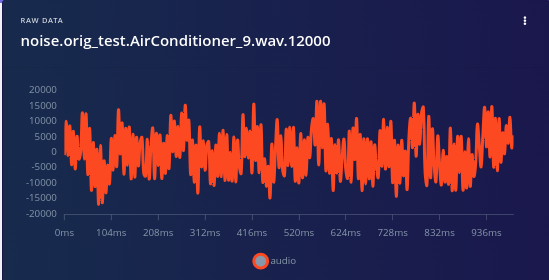
\includegraphics[width=.55\linewidth]{Img/noise.png}
    \caption{Espectro del ruido.}
    \label{noise}
    \end{figure}
\item \texttt{UNKNOWN}.
    \begin{figure}[H]
    \centering
    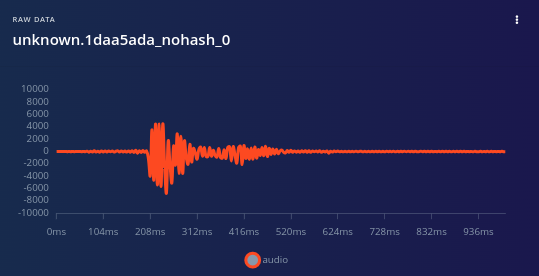
\includegraphics[width=.55\linewidth]{Img/unknown.png}
    \caption{Espectro de sonido desconocido.}
    \label{unk}
    \end{figure}
\end{itemize}
La misma plataforma ayudó a separar las grabaciones de  \SI{20}{\s} en 12 muestras. Lo que hace más rápido y sencillo el procesamiento de datos en las 2 palabras clave. Ahora, las dos etiquetas restantes fueron proporcionadas por Edge-impulse.\\
Luego, con todos los datos listos en \cite{web10} es posible realizar la clasificación de los datos.
    \begin{figure}[H]
    \centering
    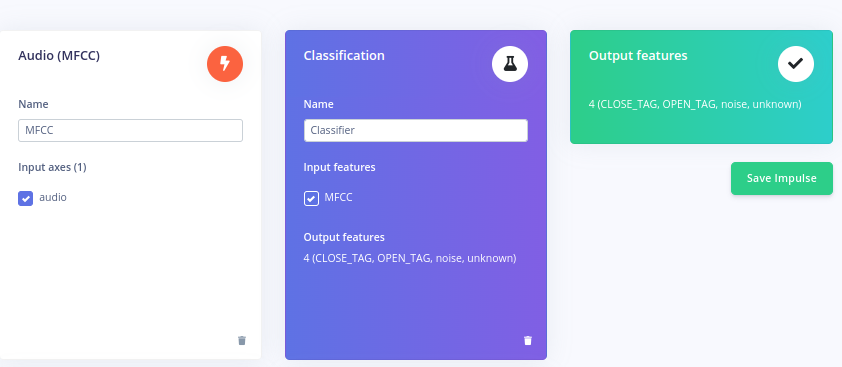
\includegraphics[width=.55\linewidth]{Img/classifier.png}
    \caption{Clasificación de los datos.}
    \label{classi}
    \end{figure}
De donde se usa una técnica de extracción de parámetros: MFCC (Mel-Frequency Cepstral Coefficientes), se definen como coeficientes cepstrales\footnote{se definen como la transformada inversa de Fourier del logaritmo del espectro de la señal de voz.} que se aplican sobre una ventana de tiempo de la señal de voz. Desde el punto de vista matemático es un operador que transforma una convolución en el tiempo en una suma espectral y de esa manera, se logran extraer los dos componentes en una señal de voz: la excitación y el tracto vocal \cite{web9}.\\
Una vez clasificados los datos, los resultados que se obtuvieron fueron los siguientes:
    \begin{figure}[H]
    \centering
    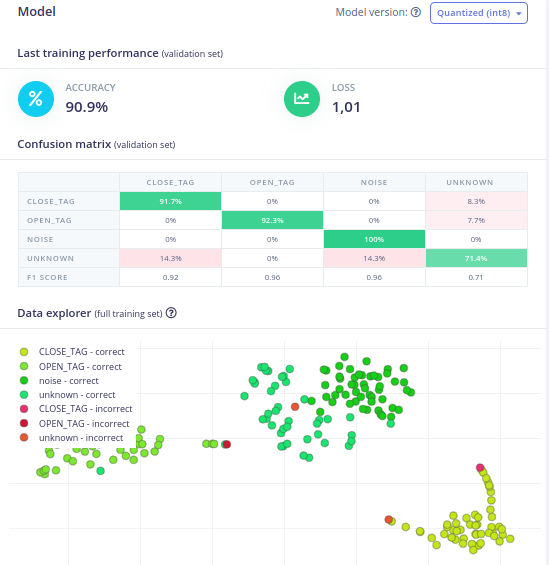
\includegraphics[width=.55\linewidth]{Img/training.png}
    \caption{Resultado fina del entrenamiento.}
    \label{training}
    \end{figure}
Por último, lo que se hizo fue configurar el \texttt{deployment} de todo lo anterior para importarlo a una librería de Arduino. Ya con esto es posible instalarla en el IDE y así editar el código conforme a las necesidades requeridas de acorde a los objetivos plantes. Es decir, que logre reconocer la palabra: \texttt{abrir} y \texttt{cierra} para activar el servomotor y así abrir o cerrar el pica-porte de una puerta, donde habrán unos LEDs que mostrarán el estado del diseño implementado.\par
Una de las primeras pruebas fue editar un poco el código generado y ver como se comportaba cuando escuchaba una de las palabras claves.

\begin{figure}[H]
   \begin{minipage}{0.48\textwidth}
     \centering
    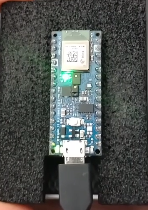
\includegraphics[width=.55\linewidth]{Img/abrir_1.png}
    \caption{Reconocimiento de la palabra abrir.}
    \label{abrir_1}
   \end{minipage}\hfill
   \begin{minipage}{0.48\textwidth}
     \centering
    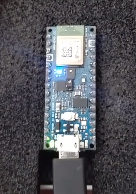
\includegraphics[width=.55\linewidth]{Img/cierra_1.png}
    \caption{Reconocimiento de la palabra cierra.}
    \label{cierra_1}     
   \end{minipage}
\end{figure}
Al decir la palabra abrir y cierra el LED del mcu muestra un color verde y azul respectivamente. También muestra un color rojo al inicio pero esto tiene que ver con la lógica que se tenía implementada.\par
Con esta comprobación fue posible hacer uso del servo motor, implementarle cierta lógica para que éste gire de 0 a 90 grados y viceversa con base al estado en el que se encuentre.
\begin{figure}[H]
   \begin{minipage}{0.48\textwidth}
     \centering
    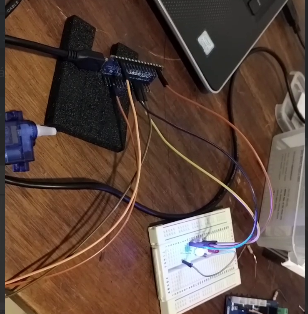
\includegraphics[width=.55\linewidth]{Img/abrir_st.png}
    \caption{Accionamiento del servo con la palabra abrir.}
    \label{abrir_st}
   \end{minipage}\hfill
   \begin{minipage}{0.48\textwidth}
     \centering
    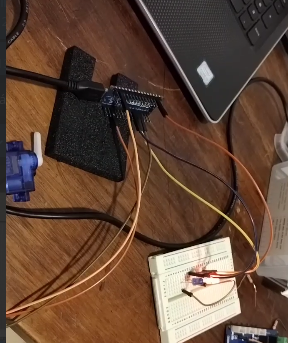
\includegraphics[width=.55\linewidth]{Img/cierra_st.png}
    \caption{Accionamiento del servo con la palabra cierra.}
    \label{cierra_st}     
   \end{minipage}
\end{figure}

Note que:
\begin{itemize}
    \item 0 grados: puerta cerrada.
    \item 90 grados: puerta abierta.
\end{itemize}
\begin{figure}[H]
   \begin{minipage}{0.48\textwidth}
     \centering
    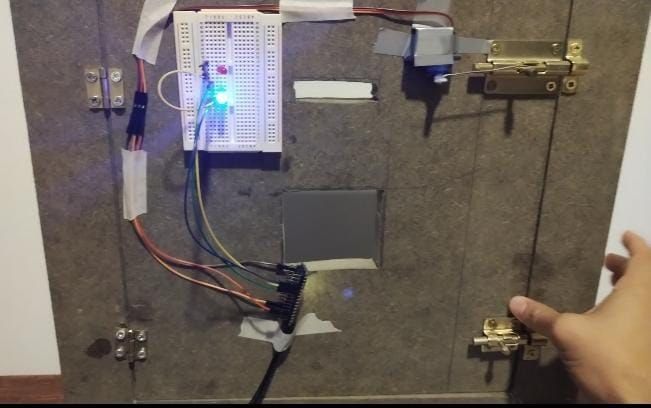
\includegraphics[width=.6\linewidth]{Img/abrir_st2.jpg}
    \caption{Funcionamiento completo con la palabra abrir.}
    \label{abrir_st2}
   \end{minipage}\hfill
   \begin{minipage}{0.48\textwidth}
     \centering
    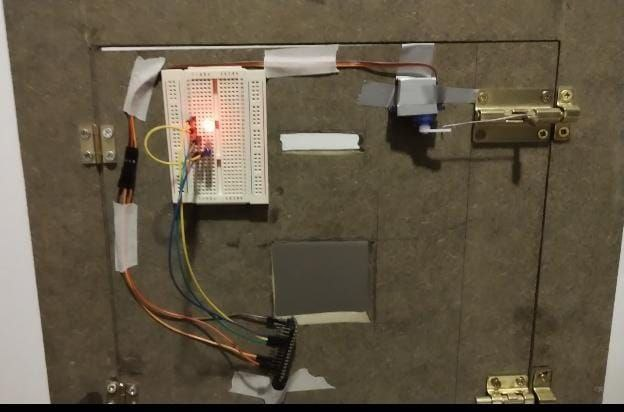
\includegraphics[width=.6\linewidth]{Img/cierra_st2.jpg}
    \caption{Funcionamiento completo con la palabra cierra.}
    \label{cierra_st2}     
   \end{minipage}
\end{figure}
Las imágenes \ref{abrir_st2} y \ref{cierra_st2} muestran el comportamiento esperado. 


%%%%%%  ¡¡¡¡¡ AQUI ME PARECE QUE VA LA SEGUNDA PARTE, FUNCIONAMIENTO COMPLETO ....!!! %%%
Una vez realizado el reconocimiento de voz, se empezó probando todos los componentes electrónicos para verificar su funcionalidad y hacer ejemplos sencillos para entender como trabajar con ellos.
La primera prueba realizada fue las del servo, en el que se utilizó la librería de ''Servo.h'' para poder manejar el mismo, es importante saber que no todos los servos tienen un mismo punto inicial, por lo que para este proyecto se tuvieron que tantear valores para poder trabajarlo de forma correcta.\\
Para el keypad se utiliza la librería de ''Keypad.h'' ya que, simplifica mucho el trabajo, simplemente es de crear una matriz que contenga los caracteres del keypad y hacer un mapeo correcto de los cables para que se detecte el carácter correcto dependiendo del botón que se pulse. Se tuvieron que hacer varias pruebas para determinar como estaba mapeado el keypad.\\
Para el lcd se decidió trabajar con un módulo de I2C, de no ser así la cantidad de cables pasaron de 8 a 4 y gracias a esto solo se tuvo que utilizar la librería de ''LiquidCrystal\_I2C.h'' y se imprimen los mensajes deseados utilizando una comunicación serial mediante el puerto USB.
Todo esto se puede observar en el siguiente enlace.
\url{https://drive.google.com/file/d/1F8vAwWyKLxurYiivwDr2JWspp3p14MrM/view?usp=sharing}
Una vez comprobado el funcionamiento de todo lo utilizado se procedió a ensamblar todo junto con la puerta, el resultado final se observa en las siguientes imagenes:
\begin{figure}[H]
    \centering
    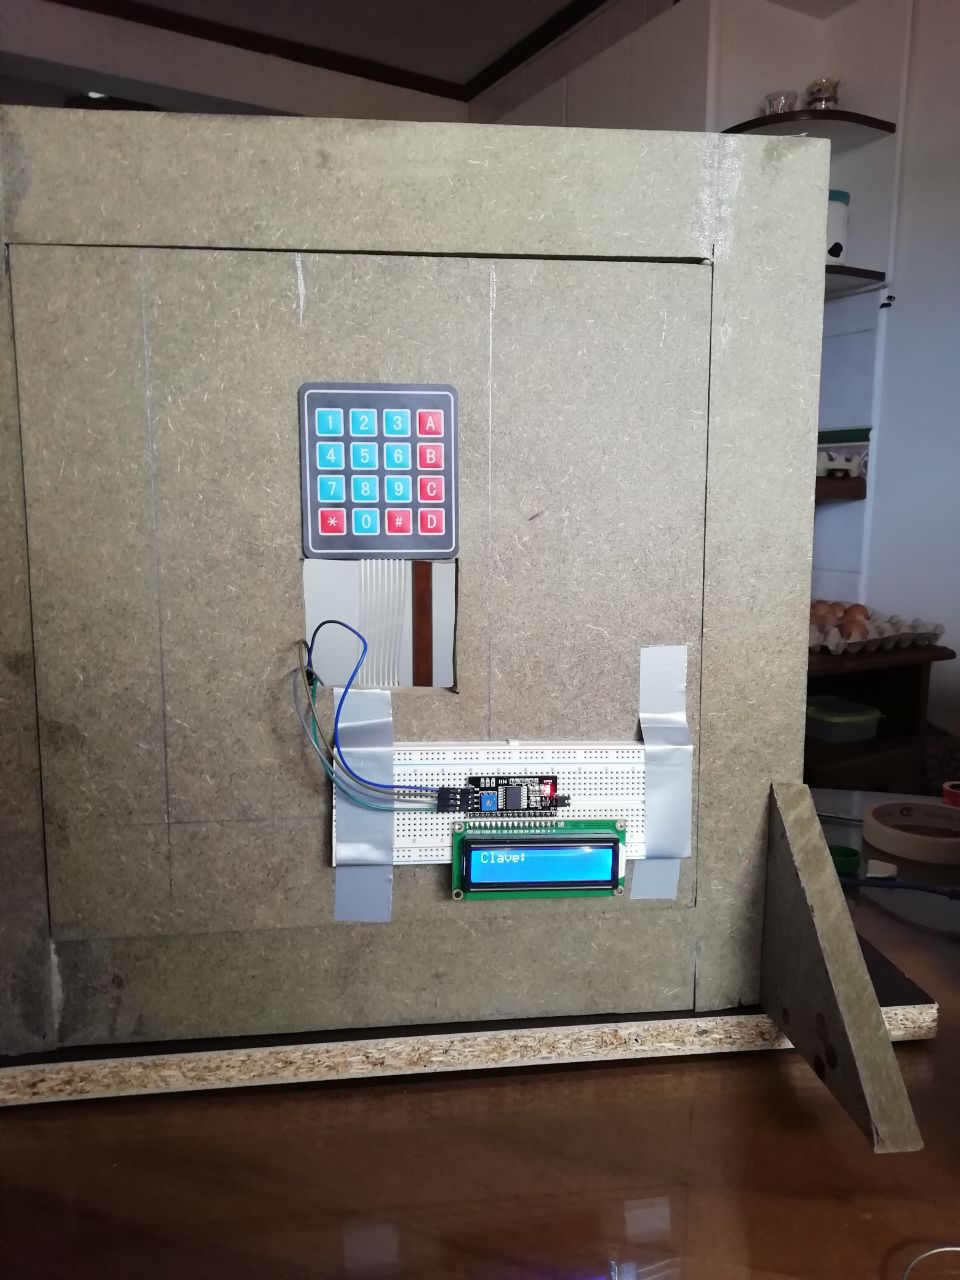
\includegraphics[width=.55\linewidth]{Img/FinalFrente.jpeg}
    \caption{Cerradura final ensamblado parte frontal.}
\end{figure}

\begin{figure}[H]
    \centering
    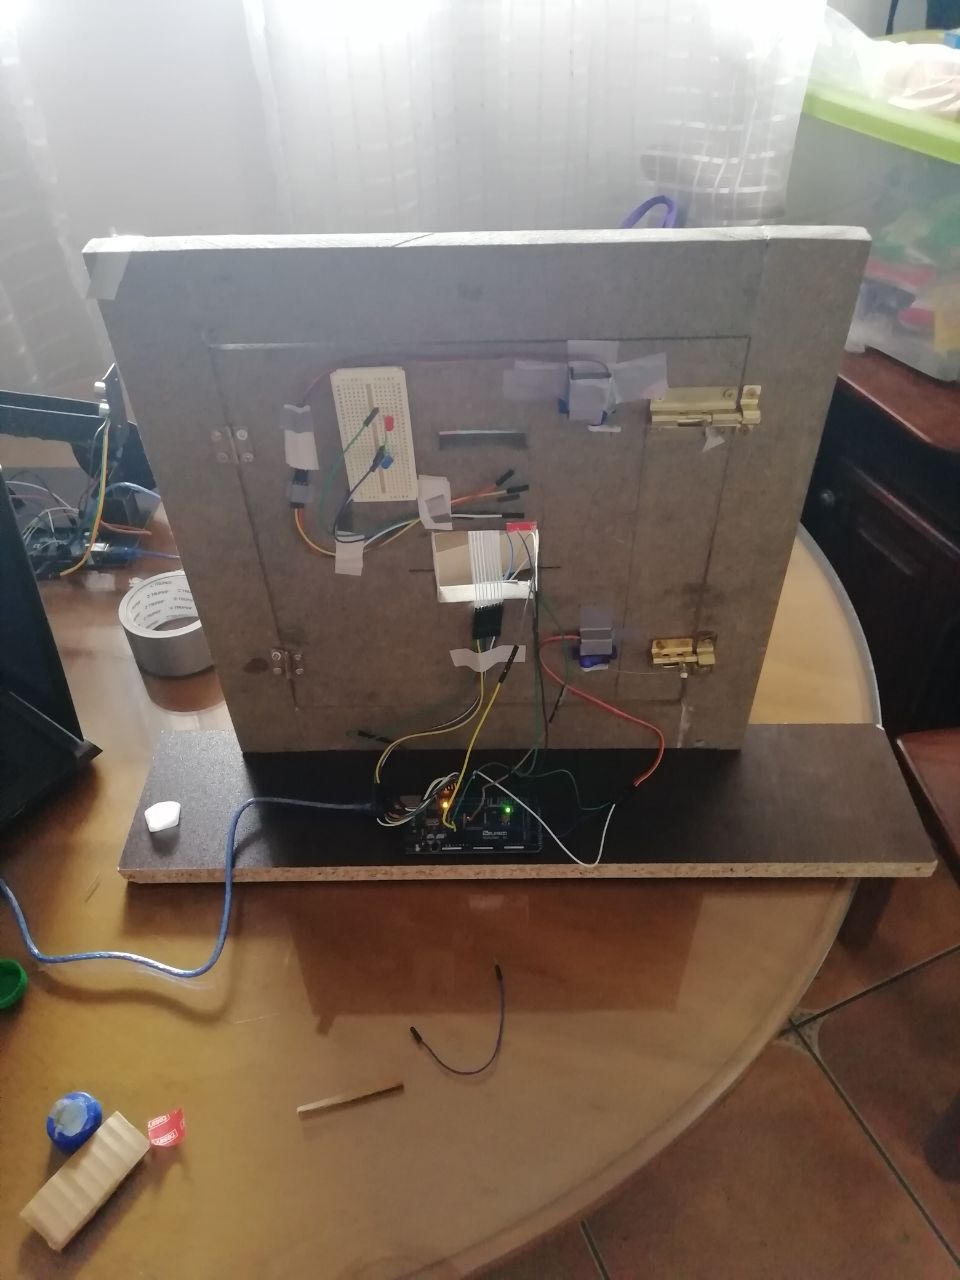
\includegraphics[width=.55\linewidth]{Img/FinalTrasero.jpeg}
    \caption{Cerradura final ensamblado parte trasera.}
\end{figure}




\newpage